\section{Evaluation}

\subsection{Experimental Settings}
Training strictly leverages batch-based operations (batch size of 128 items from the PyTorch DataLoader) mapping cleanly into our matrix dot products. The Multi-Layer Perceptron (MLP) was comprehensively evaluated over 30 epochs employing a foundational learning rate ($\eta$) of 0.5, while the CNN traversed its localized feature extraction mapping utilizing fine-tuned constraints. 

\subsection{Training Progression and Feature Extraction}
As observed in our empirical metrics, the model displays robust convergence stability. The Cross-Entropy loss smoothly decays while overall Test Accuracy steadily rises, breaking past 90\% accuracy thresholds within limited iterations (Figure \ref{fig:curves}).

\begin{figure}[htbp]
    \centering
    \begin{minipage}{0.48\textwidth}
        \centering
        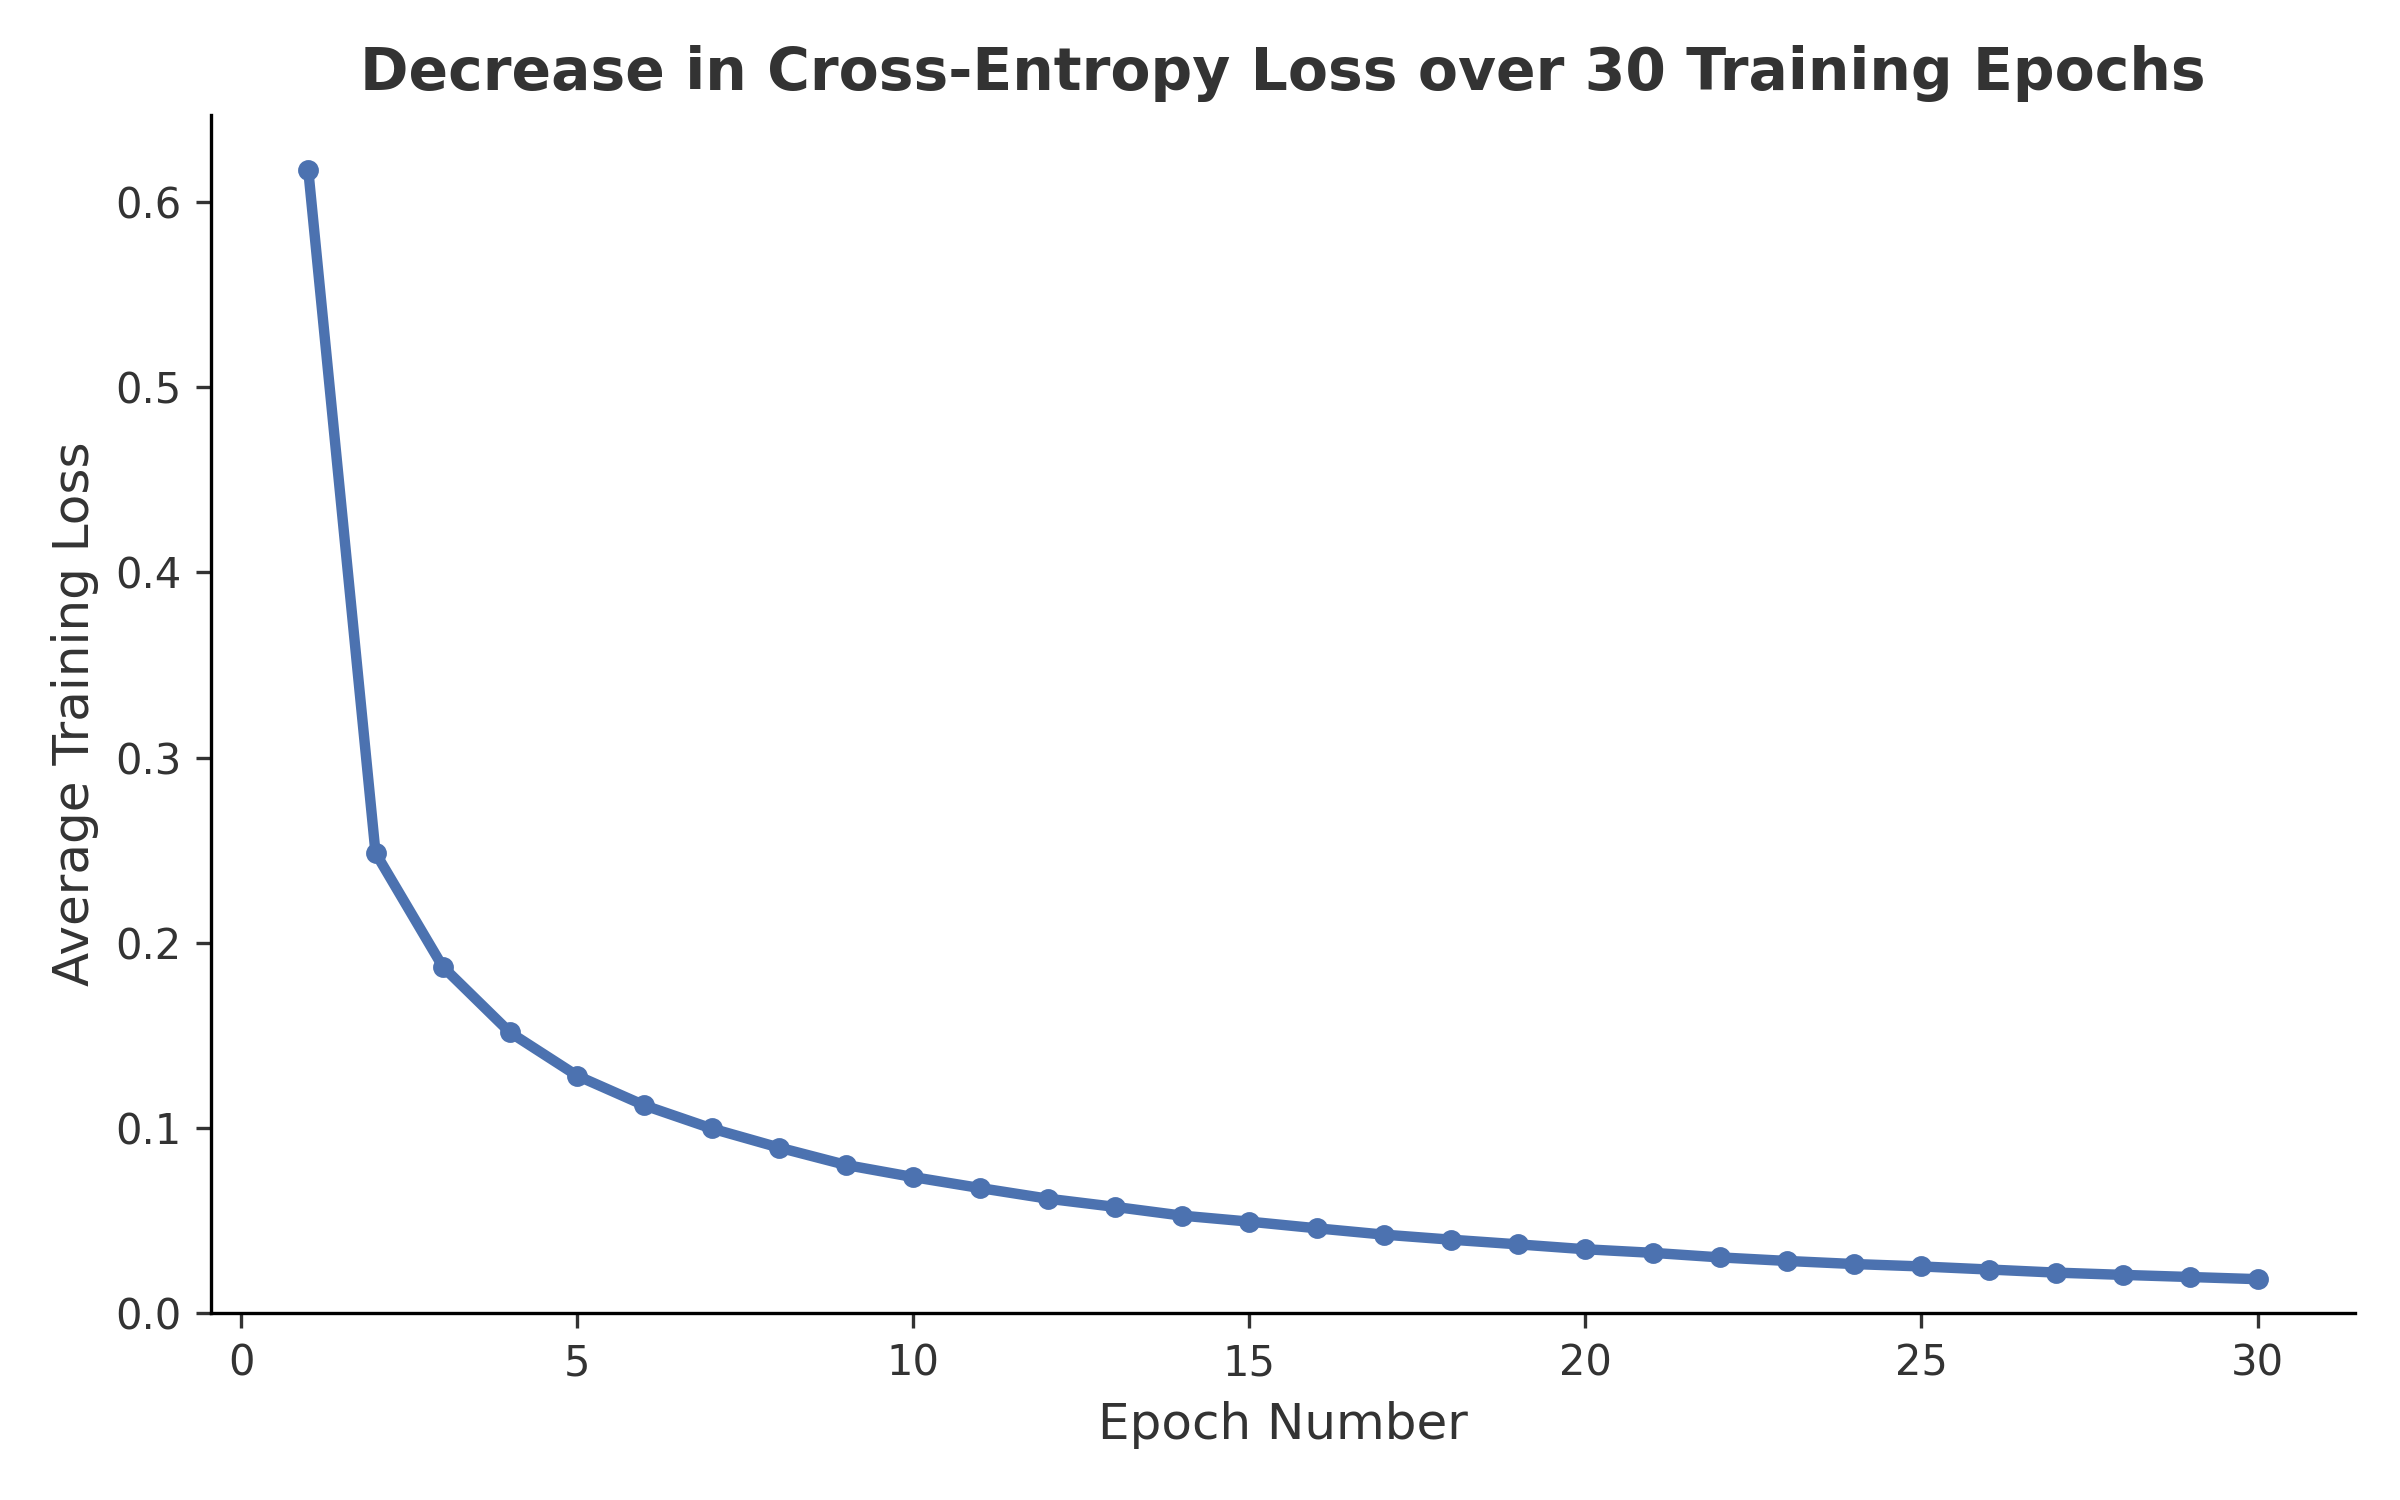
\includegraphics[width=\textwidth]{images/MLP/curves/training_loss_curve.png}
        \caption{Decrease in Cross-Entropy Loss (MLP)}
    \end{minipage}\hfill
    \begin{minipage}{0.48\textwidth}
        \centering
        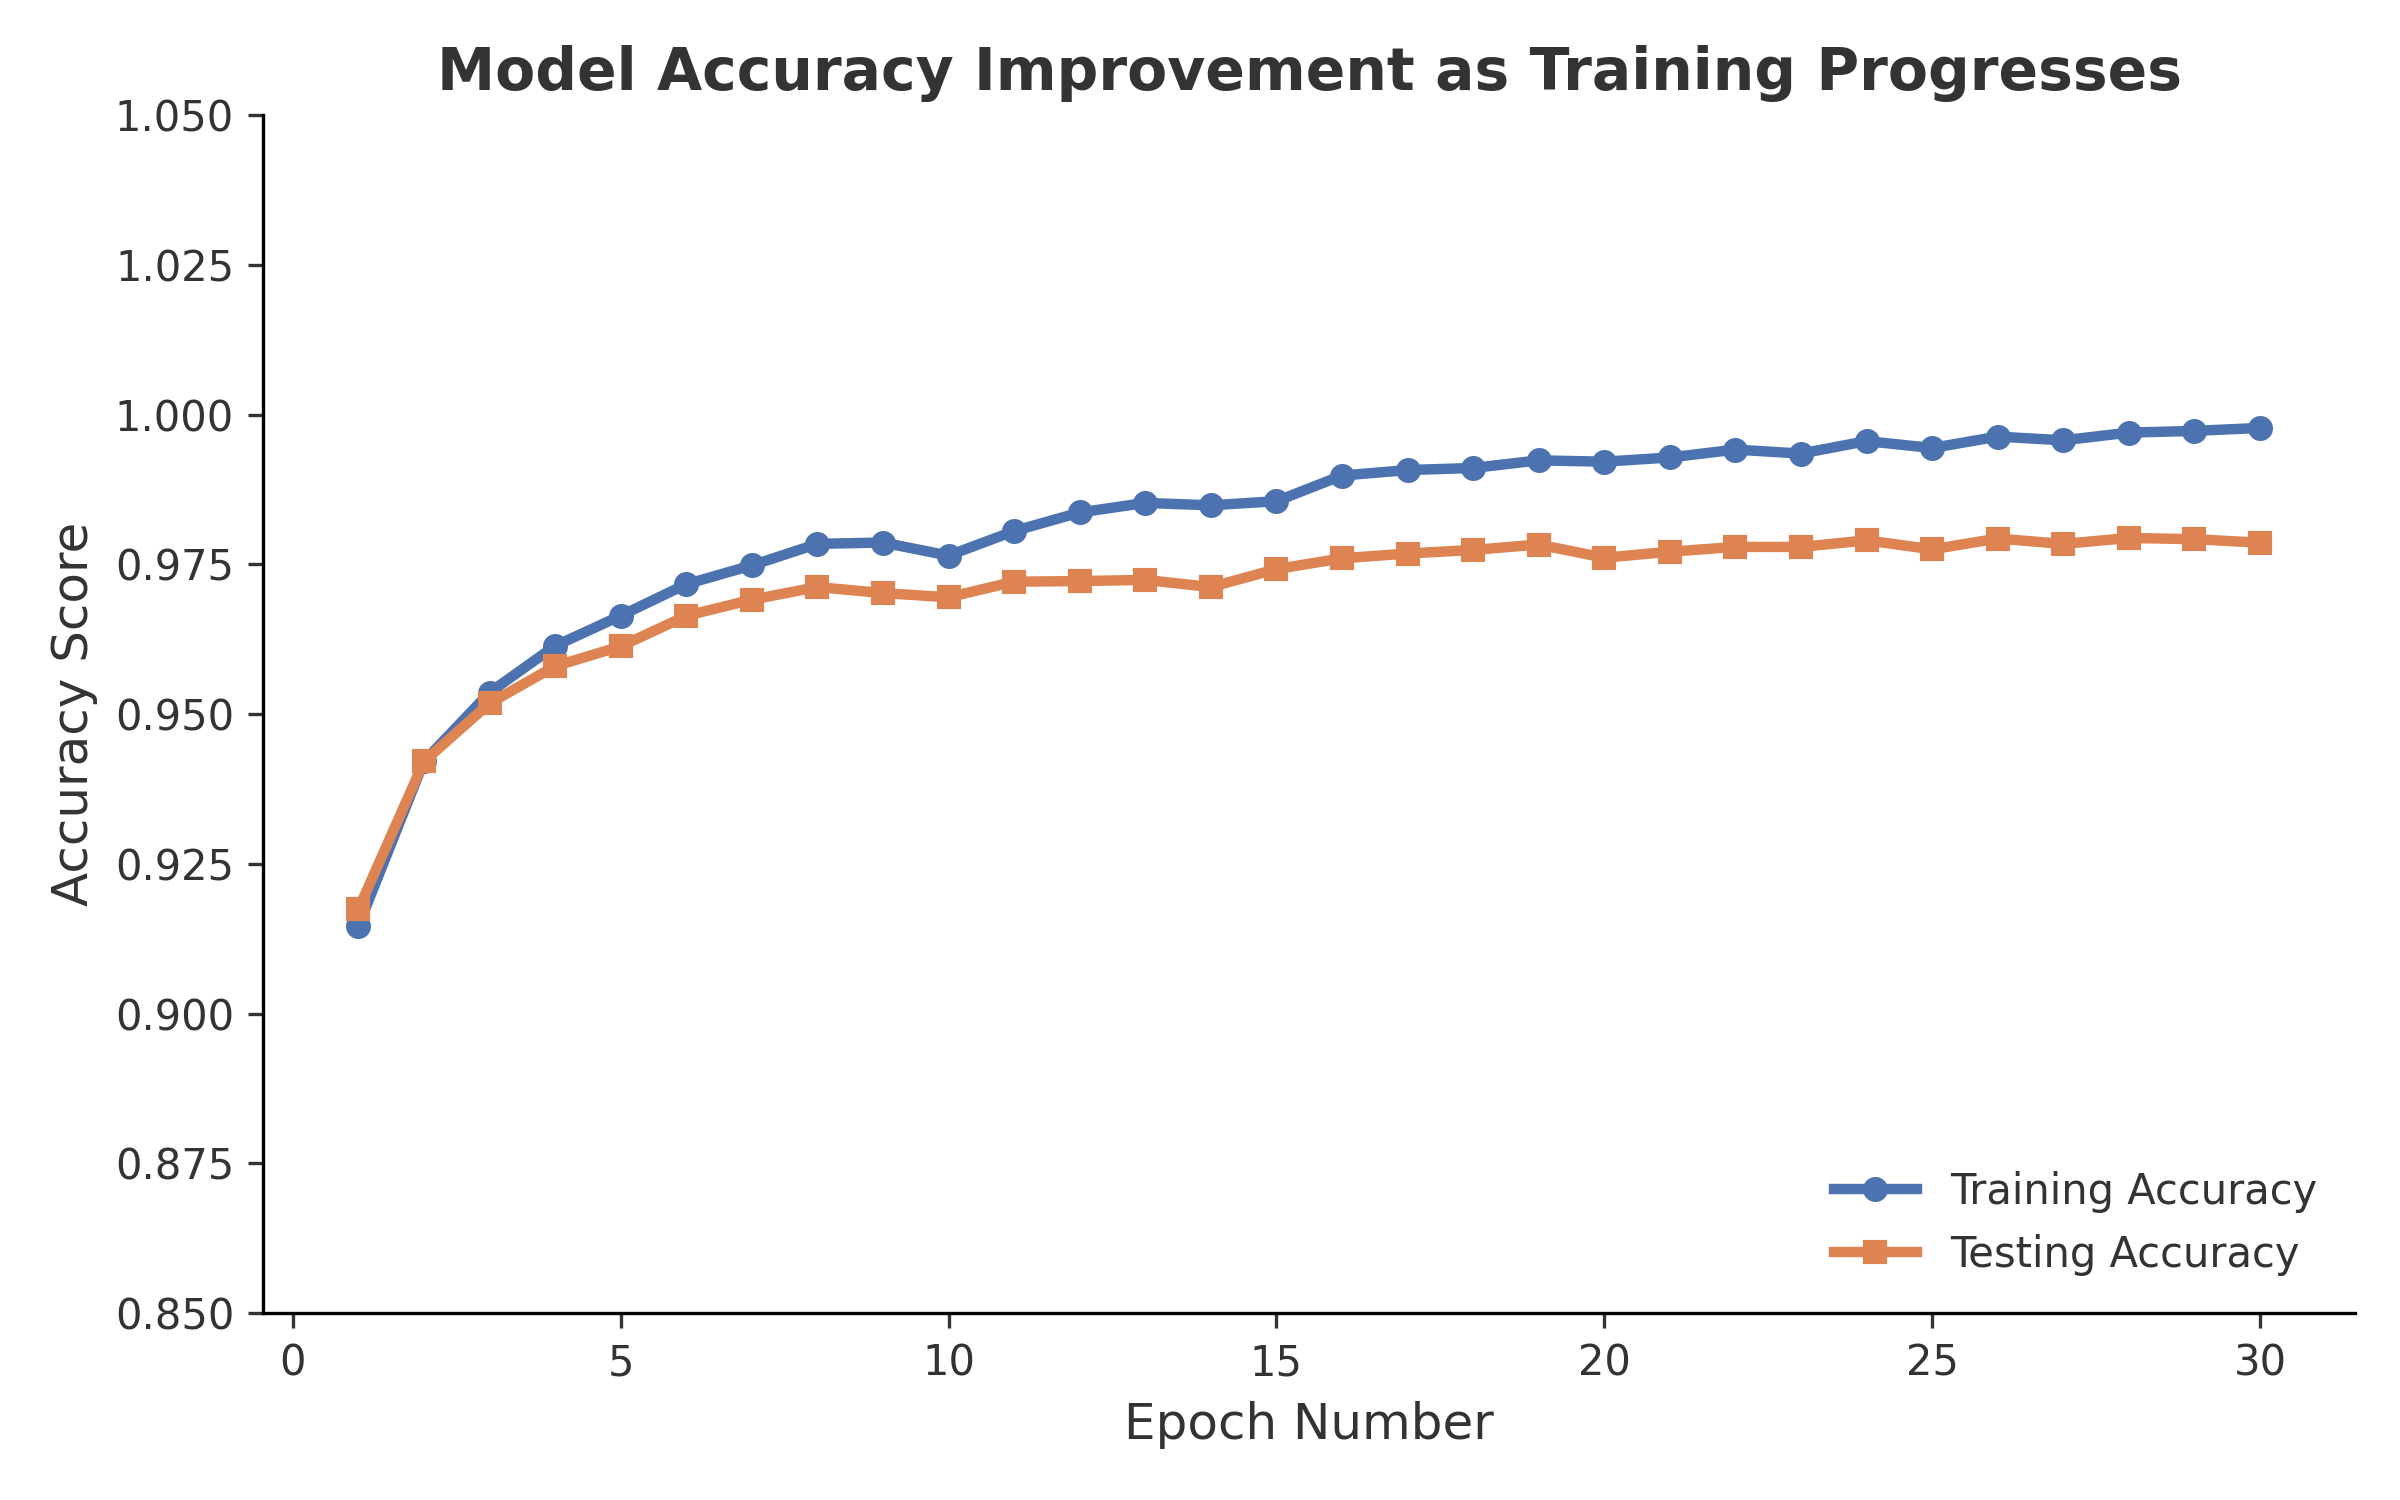
\includegraphics[width=\textwidth]{images/MLP/curves/accuracy_curve.png}
        \caption{Accuracy trajectory indicating no severe overfitting}
        \label{fig:curves}
    \end{minipage}
\end{figure}

Delving deeper into feature extraction, evaluating the 128 hidden neurons provides remarkable intuition regarding the mapping characteristics generated by the model. 

\begin{figure}[htbp]
    \centering
    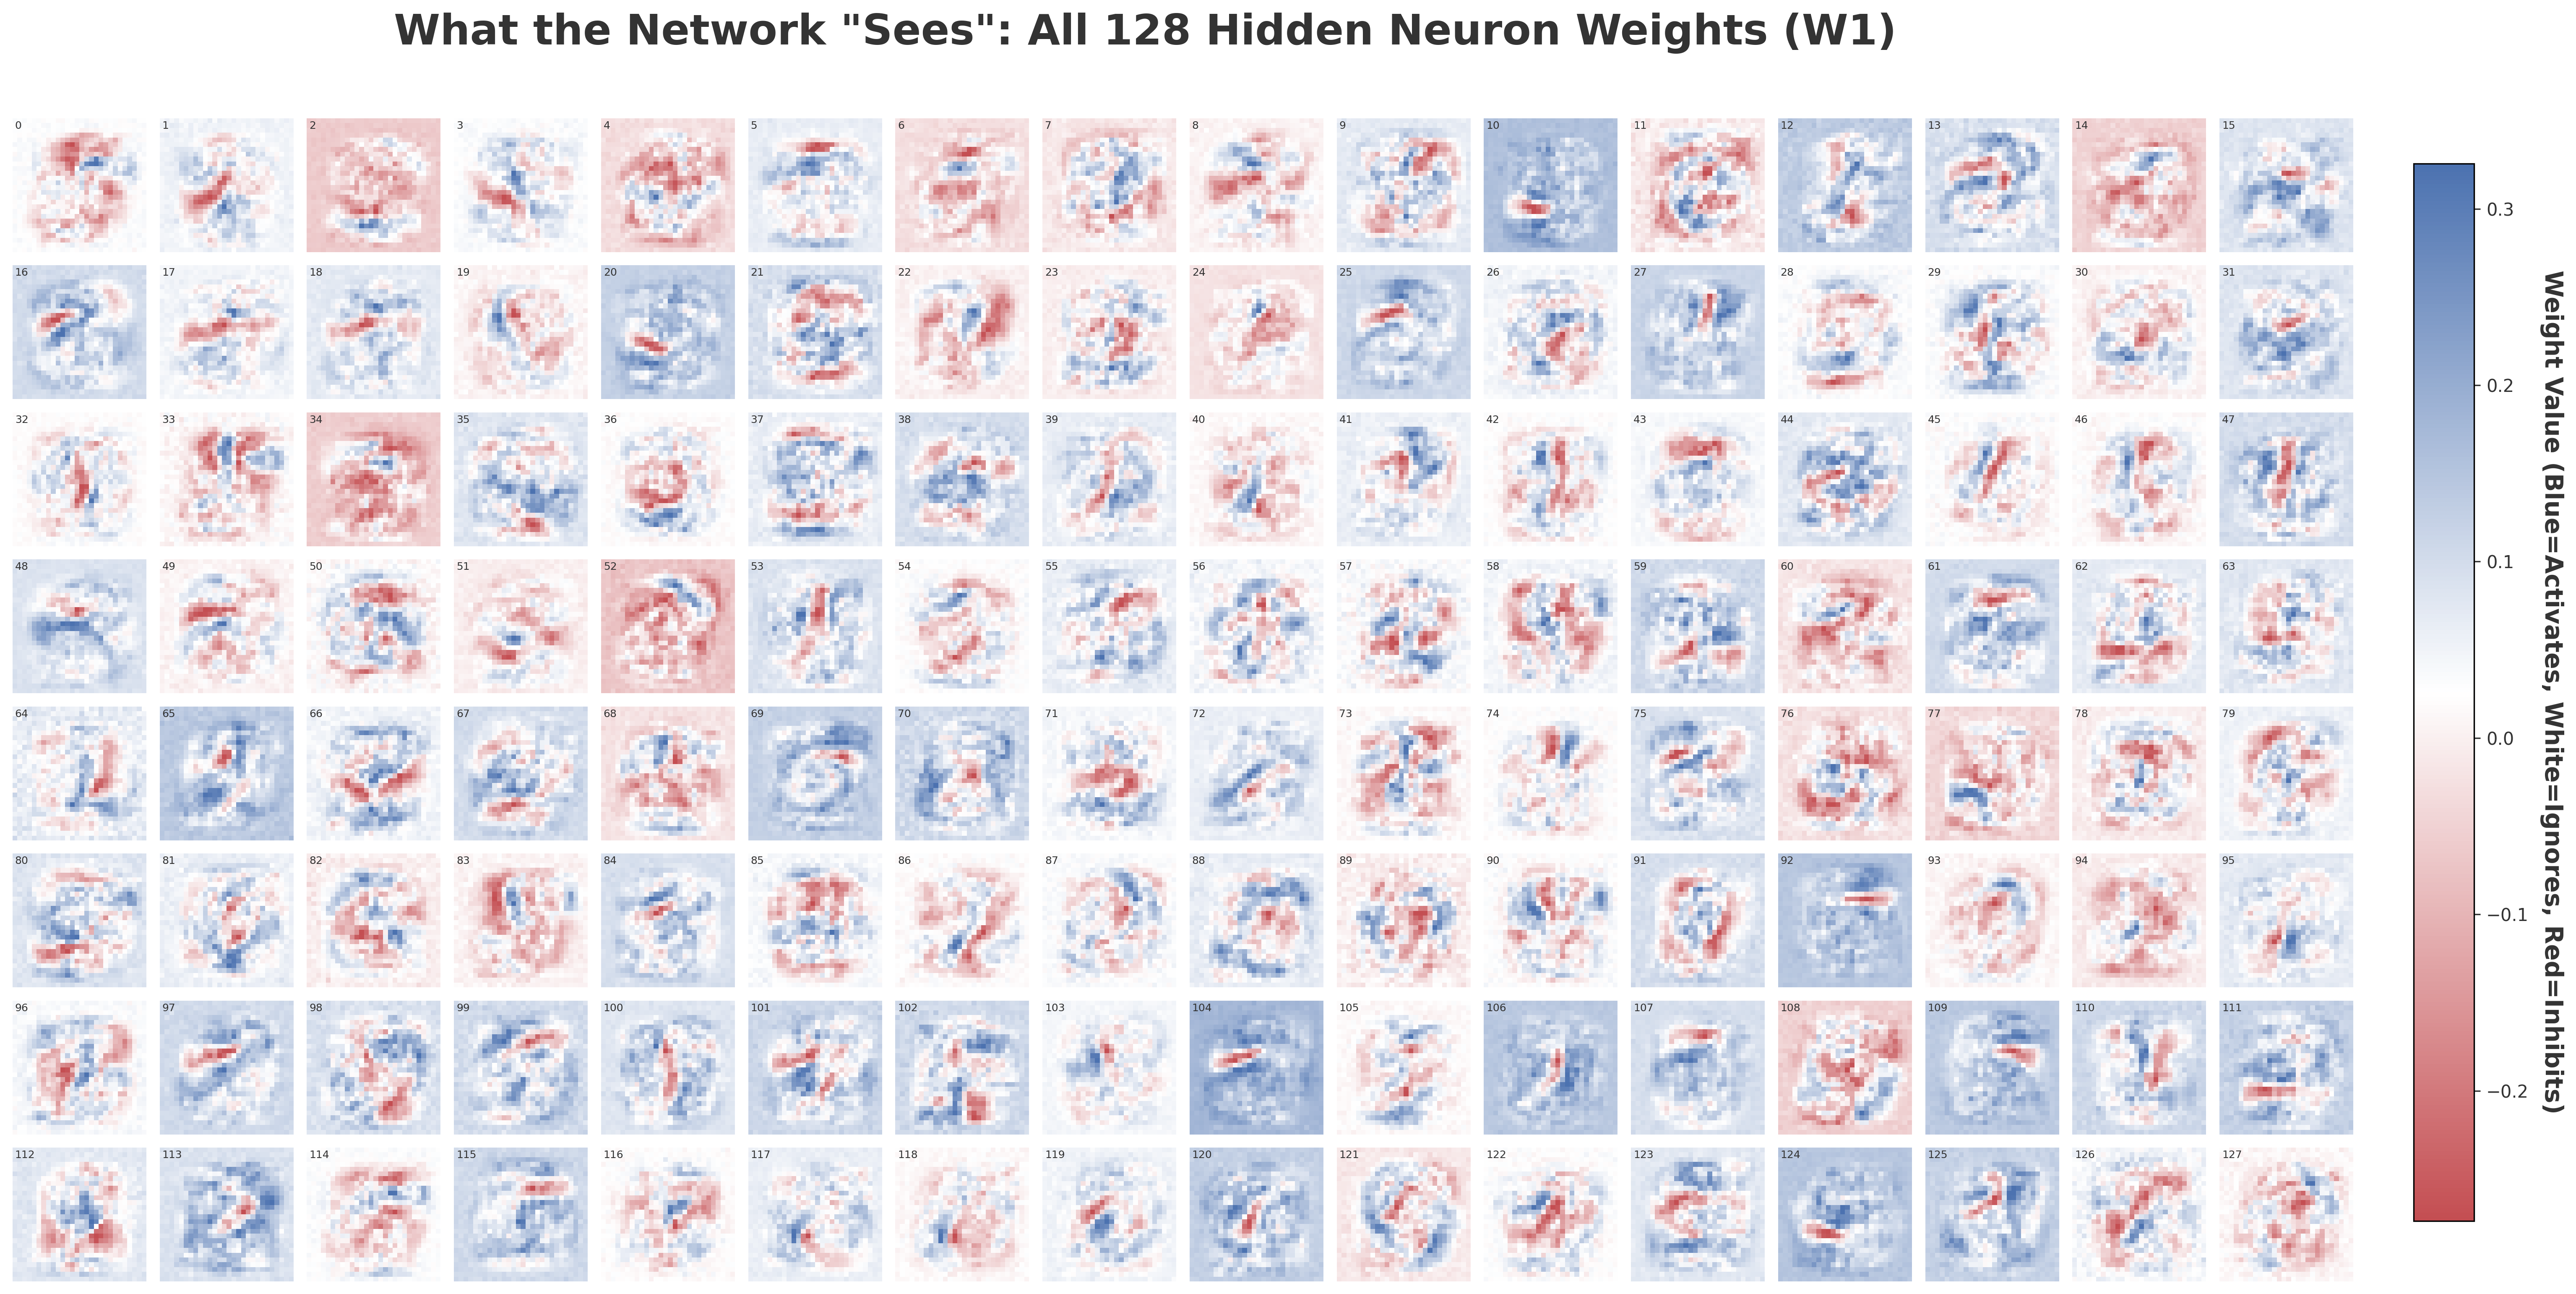
\includegraphics[width=\textwidth]{images/MLP/weights/all_128_learned_weights.png}
    \caption{Representation of learned weights across all 128 Hidden Neurons in W1. Organized as a $8\times 16$ lattice directly corresponding to hidden layer activations.}
\end{figure}

\subsection{Qualitative Profiling and Confusion Analysis}
Sample step-by-step predictions visually validate the model's forward propagation fidelity (Figure \ref{fig:stepbystep}). 

\begin{figure}[htbp]
    \centering
    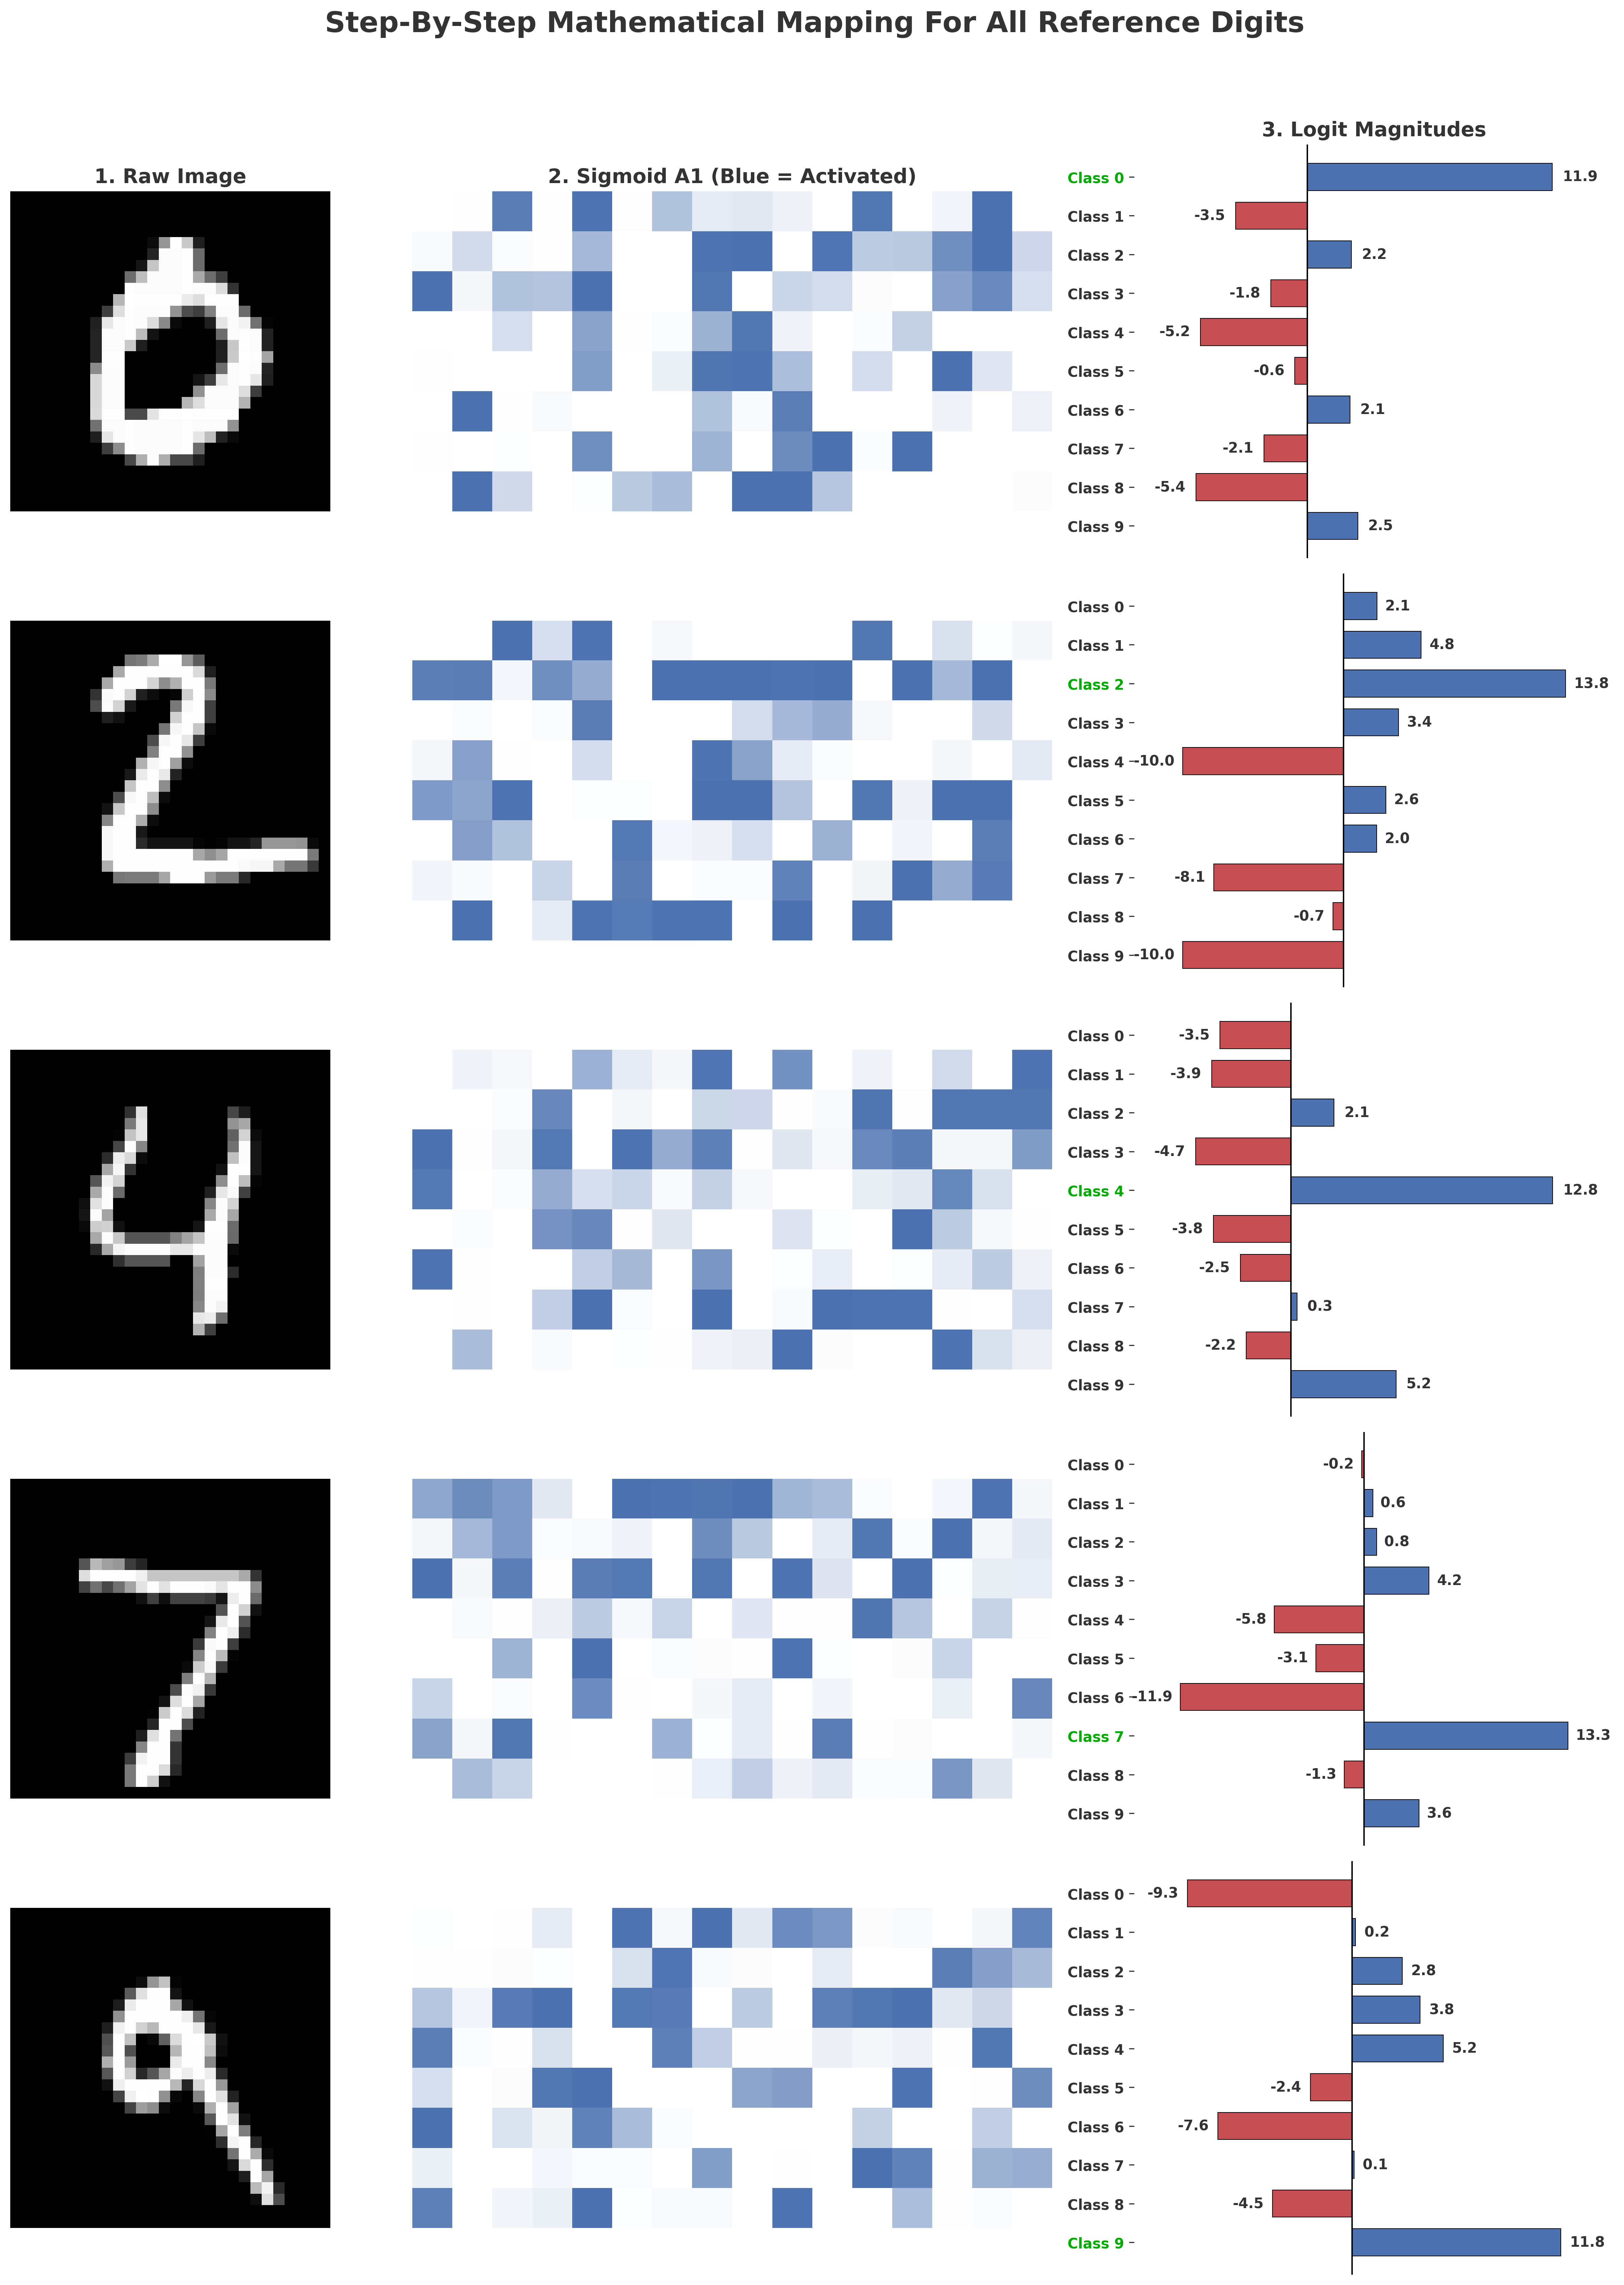
\includegraphics[width=0.9\textwidth]{images/MLP/sample/forward_propagation_reference_steps.png}
    \caption{Manual inspection illustrating exact network representations (Input, Hidden map, and Logits) for a subset of global reference digits.}
    \label{fig:stepbystep}
\end{figure}

To definitively document overall performance barriers, the model's total interactions across 10,000 distinct test samples were synthesized within a detailed semantic Confusion Matrix (Figure \ref{fig:cm}). Additionally, hyperparameter analysis confirms that shifting the quantity of allocated hidden neurons directly correlates with capacity breakpoints scaling network accuracy (Figure \ref{fig:ne_bench}).

\begin{figure}[htbp]
    \centering
    \begin{minipage}{0.48\textwidth}
        \centering
        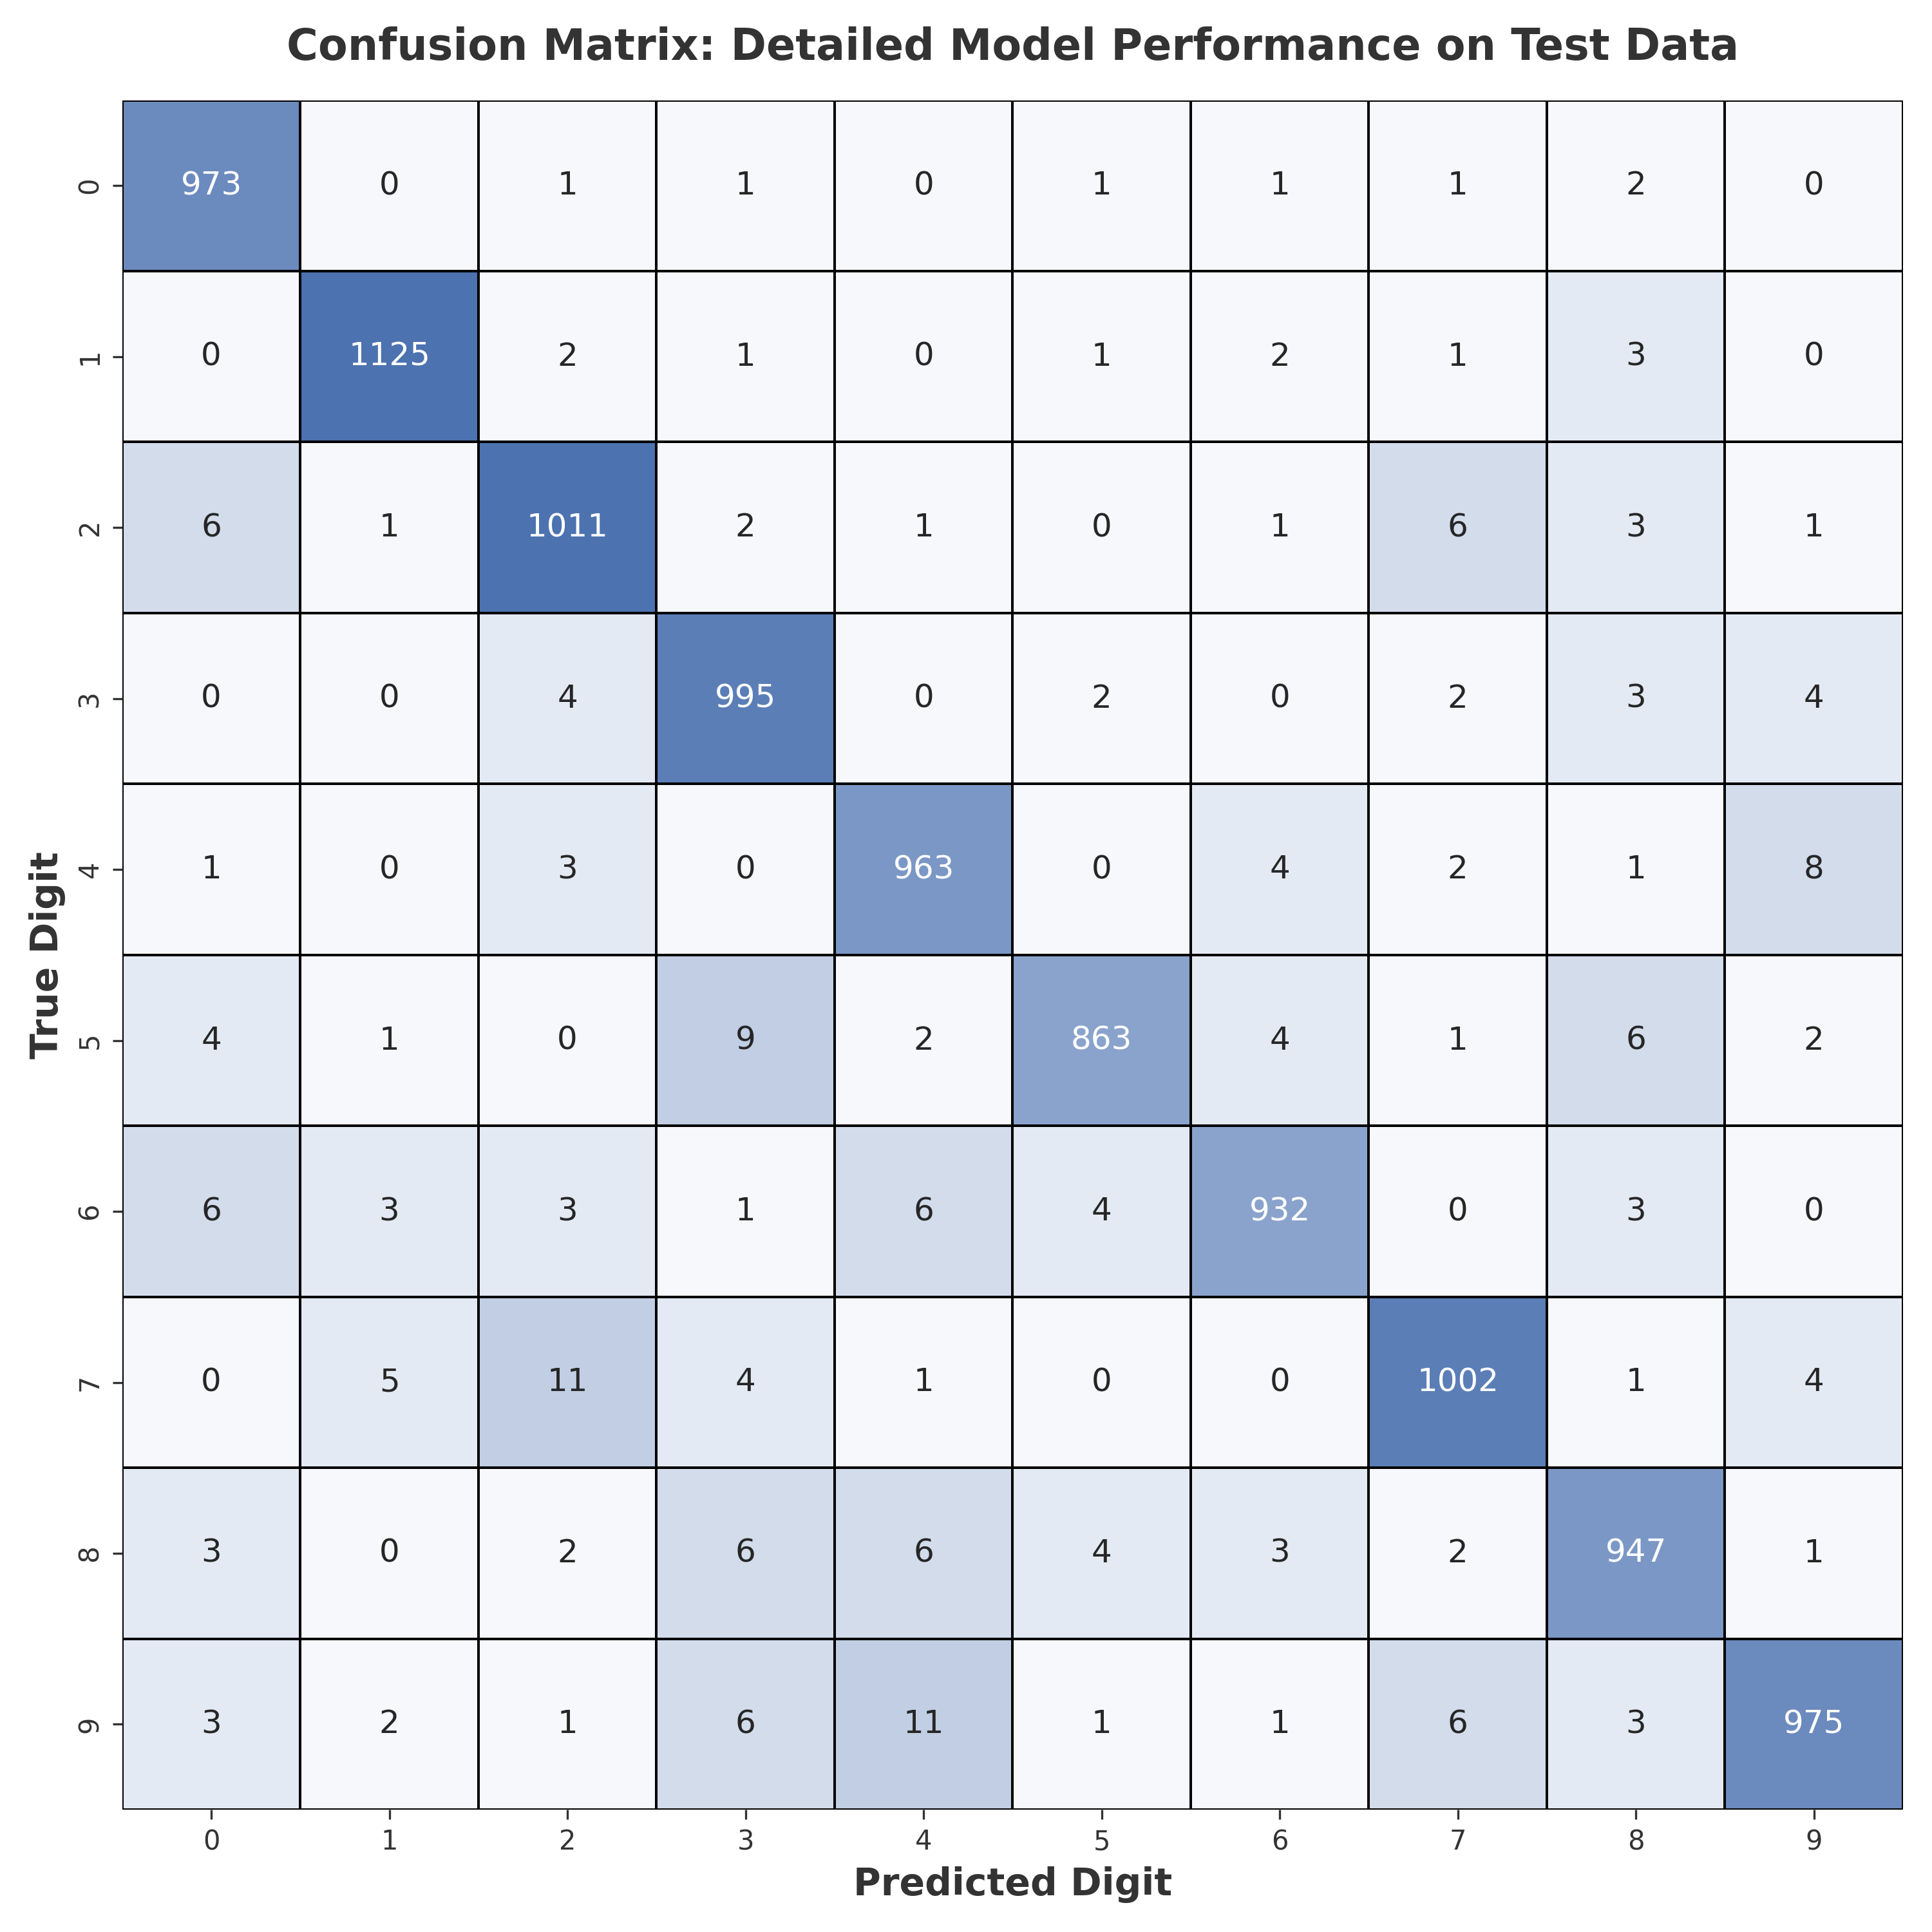
\includegraphics[width=\textwidth]{images/MLP/errors/confusion_matrix.png}
        \caption{Evaluation of Test Predictions (Confusion Matrix)}
        \label{fig:cm}
    \end{minipage}\hfill
    \begin{minipage}{0.48\textwidth}
        \centering
        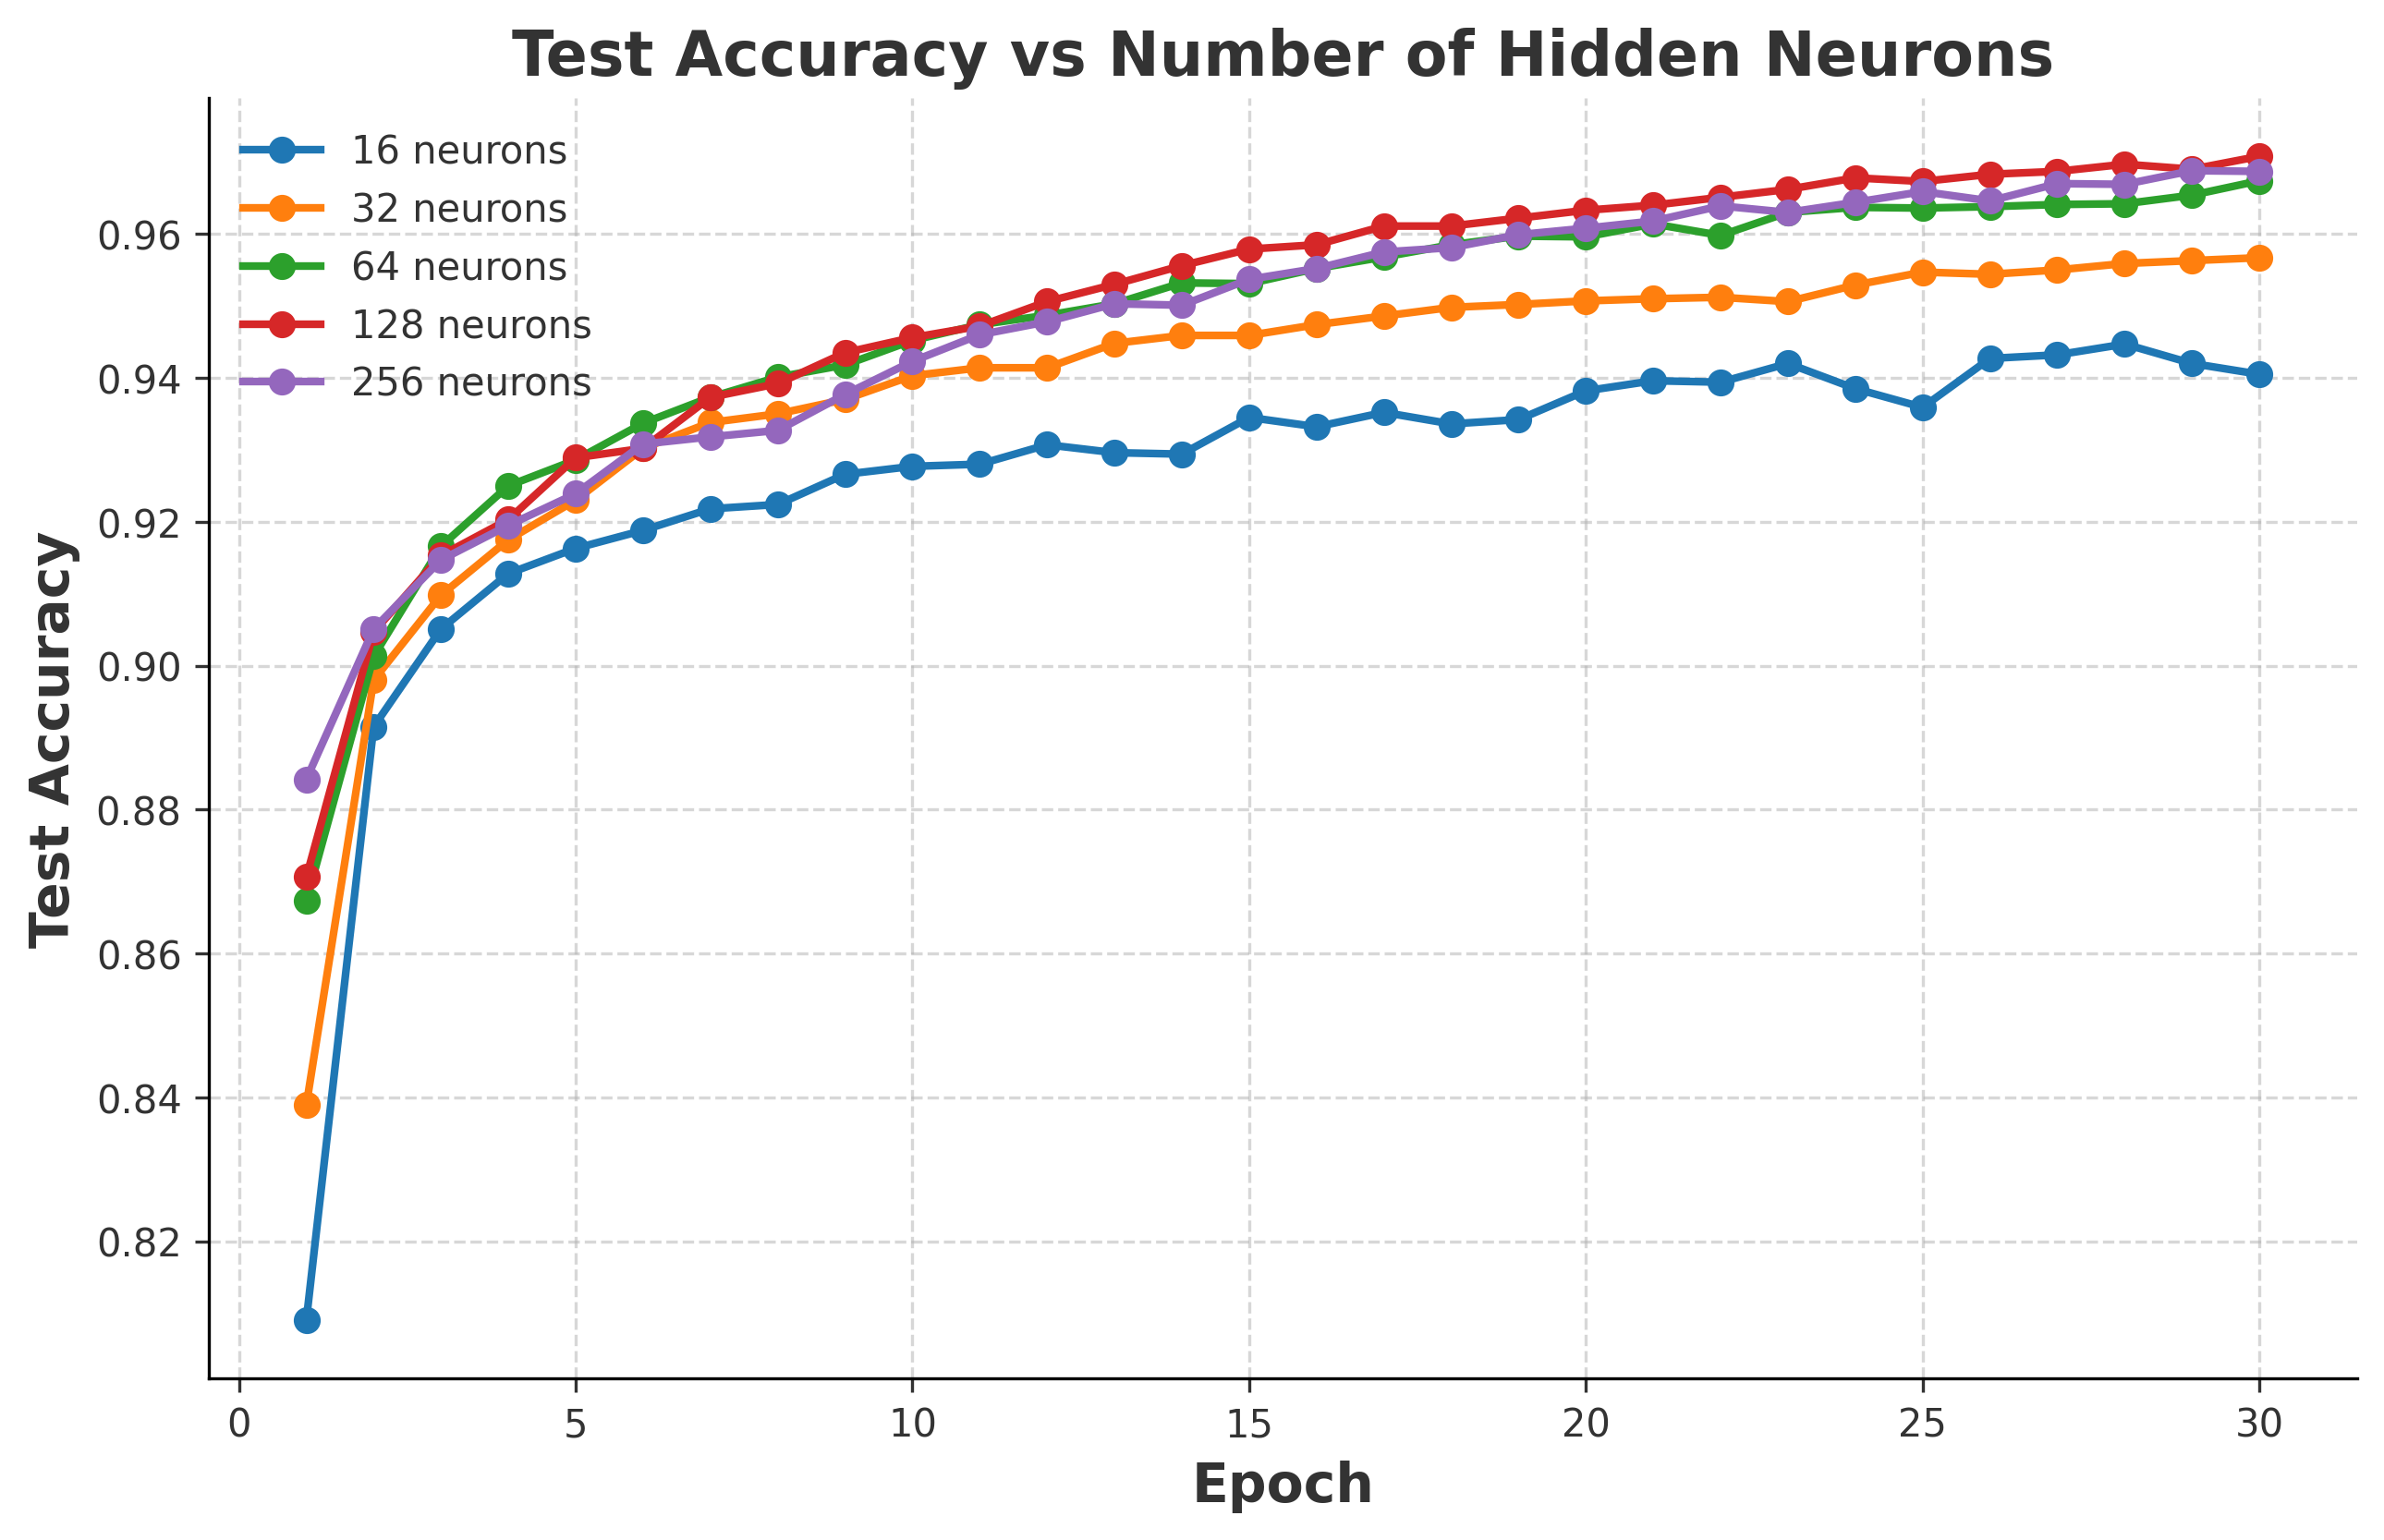
\includegraphics[width=\textwidth]{images/MLP/curves/neuron_comparison.png}
        \caption{Impact of Hidden Neuron Counts on Test Accuracy}
        \label{fig:ne_bench}
    \end{minipage}
\end{figure}
